\chapter{Background}
\label{Background}
There are many scenarios on the web which can result in the loss of user information or harm to the browsing device. These include phishing pages, pages infected with malware or other unwanted software, and the insecure transmission of sensitive information. Each of these scenarios can be dangerous for users and thus should generally be avoided.

Modern web browsers attempt to mitigate risk by displaying firm and assertive warning messages when a page is suspected to be dangerous (see figure \ref{fig:Warning-Firefox-SSL}). Unfortunately, many studies on the effectiveness of such messages have been conducted in the past and results have generally been poor. Users frequently ignore browser warnings and put themselves at risk nonetheless. Felt et al. \cite{felt2015improving} found that the rate of warning dismissal is 38\% in the case of Google Chrome’s SSL warning and in a study conducted by Sunshine et al. \cite{sunshine2009crying}., once participants learned how to ignore a warning in one situation, they typically ignored the warning in future encounters as well.

\begin{figure}[th]
	\centering
	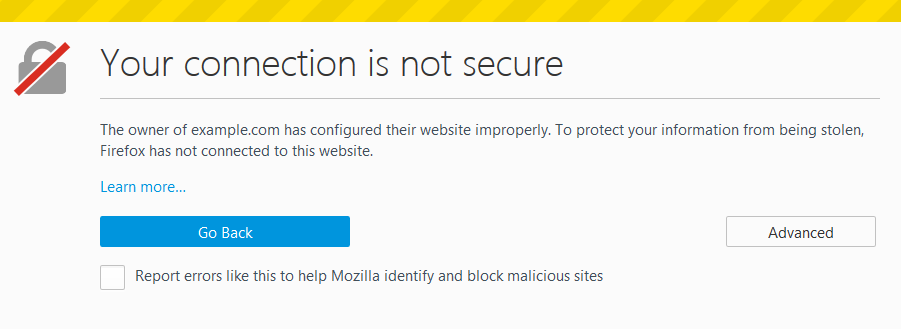
\includegraphics[width=\textwidth]{Figures/Warning-Firefox-SSL}
	\decoRule
	\caption[Firefox's SSL warning]{Firefox's SSL warning in Firefox version 52.}
	\label{fig:Warning-Firefox-SSL}
\end{figure}

Habituation is often identified by researchers as a critical reason for warning dismissal. \cite{akhawe2013alice, egelman2008warned}. Anderson et al. \cite{anderson2015polymorphic} investigated habituation at the neurological level and conducted a study which examined participants' brains in an fMRI machine while observing warning messages. They found that the effects of habituation could be seen after as few as two viewings of a given warning message. They were able to combat this phenomenon and significantly reduce the effects of habituation by using polymorphic, appearance-changing warning messages.

With this in mind, since similar looking warning messages are used in different situations, it is possible that the current approach to browser warning messages does not effectively convey important information. Understanding may instead be diluted by treating all warnings as equally severe. In this study, we investigate the impact of using tiered warning messages to alert users.

User understanding of risks is a key factor in adherence to warning messages. As has been found by Almuhimedi and Felt \cite{almuhimedi2014reputation} and Dhamija et al. \cite{dhamija2006phishing}, users generally ignore warnings because they do not understand the risks, or they trust the page they are attempting to visit and believe the warning was issued in error (i.e., a false positive). In the study conducted by Sunshine et al. \cite{sunshine2009crying}, some participants confused SSL warning messages with 404 pages, thinking that the server they were trying to access was down or somehow blocked. Thus, in addition to adherence rates, it is also of interest to know which \emph{aspects} (if any) of our tiered warning messages draw the attention of participants and if they truly understand the risks (not solely that any given warning as a whole is adhered to more or less frequently).
